\documentclass[hidelinks]{article}
\usepackage[utf8]{inputenc}
\usepackage[a4paper, margin=3cm]{geometry}
\usepackage{algorithm, algpseudocode, amsmath, amssymb, amsthm, mathtools}
\usepackage{caption, comment, enumerate, float, graphicx, harmony, hyperref, listings, multicol, soul}
\usepackage{tikz}
\usepackage{xcolor, xfrac}

\usetikzlibrary{arrows, shapes, fit}
\tikzset{
  treenode/.style = {align=center, inner sep=0pt, text centered, font=\sffamily},
  arn_n/.style = {treenode, circle, white, font=\sffamily\bfseries, draw=black, fill=black, text width=2.5em},
  arn_r/.style = {treenode, circle, red, draw=red, text width=2.5em, very thick},
}

\renewcommand{\comment}[2]{#2}
\newcommand*{\figuretitle}[1]{
    {          
        \centering
        \textbf{#1}
        \par\medskip
    }
}

%Begin van het document
\begin{document}

\section*{Introduction}
This document has as purpose to serve as an exercise for you to try out some things within \LaTeX\; for each level individually. At the end there are also some challenges if you think you got what it takes. Good luck in recreating this document!

\clearpage

\section*{Beginner}
$\Big((\neg A\Rightarrow B) \vee (C \wedge D)\Big) \leftrightarrow E $

\begin{tabular}{| c c c |}
1 & 2 & 3\\
\hline
4 & \multicolumn{2}{c|}{5} \\
6 & 7 & $\alpha$
\end{tabular}\\

Question! Is dark mode better than light mode?
\begin{enumerate}[a)]
	\item Yes
	\item No
\end{enumerate}

Maybe I \textit{want} to create a \textbf{table}$\cdots$\\

Or maybe \qquad just \qquad some \st{words} that are {\Huge VERY} important.

\[f(x) = \frac{1}{2}\cdot\binom{4}{1}\]
\[f_{2}(x) = \int_{a}^{b}x^2\]

A nice $\AAcht$ perhaps? Please visit \url{youtube.com}

\clearpage

\section*{Intermediate}
L\"{e}t's g\'{o}¡\\[5mm]
\begin{minipage}{0.5\textwidth}
Hello\dots
\begin{equation*}
	\alpha(z_{1}, z_{2}) = \left(\dfrac{\partial\beta(z_{1}, z_{2})}{\partial z_{1}}, \dfrac{\partial\beta(z_{1}, z_{2})}{\partial z_{2}}\right)
\end{equation*}
\vfill
\end{minipage}
\begin{minipage}{0.5\textwidth}
Is it me you're looking for?
\begin{align*}
\vec{v} &= 
\begin{pmatrix}
	\lambda & 0 \\
	0 & \lambda \\
\end{pmatrix}
\\
&= \lambda\cdot \text{I}
\end{align*}
\end{minipage}

Clearly the complexity of this algorithm is $\mathcal{O}\left(n\log n\right)$, as is given by the following:

\begin{lstlisting}[frame=single]
    private void smartMethod() {
        Operator op = new Operator(nr_of_questions, input);
        if (input.size() < 3) {
            op.low_students();
            answers = op.getAnswers();
        } else if (op.correct_input()) {
            op.smartSolution();
            answers = op.getAnswers();
        } else {
            answers.add((long) 0);
            answers.add((long) 0);
        }
    }
\end{lstlisting}

Given is that $\forall\eta,\exists\pi\in\mathbb{C}$ such that $\gamma(\boldsymbol{\eta}) \stackrel{?}{=}
\begin{cases}
	0 & \text{ if } \eta=0\\
	\displaystyle\max_{i\geq5}\left[\dfrac{\pi}{\lambda}\right] & \text{ if }\eta>0\\
\end{cases}$

\begin{figure}[H]
	\textbf{Little bit wrong}
	\centering
	
\includegraphics[height=7cm, width=5cm]{Images/svCognAC}
	\caption{This is COGNAC!}
\end{figure}

\clearpage

\section*{Advanced}
-

\clearpage

\section*{Expert}
-

\clearpage

\section*{Godlike}
-

\clearpage

\section*{Challenges}
Tip: I created these images with the Tikz package from scratch, so they are created solely in \LaTeX!
\begin{center}
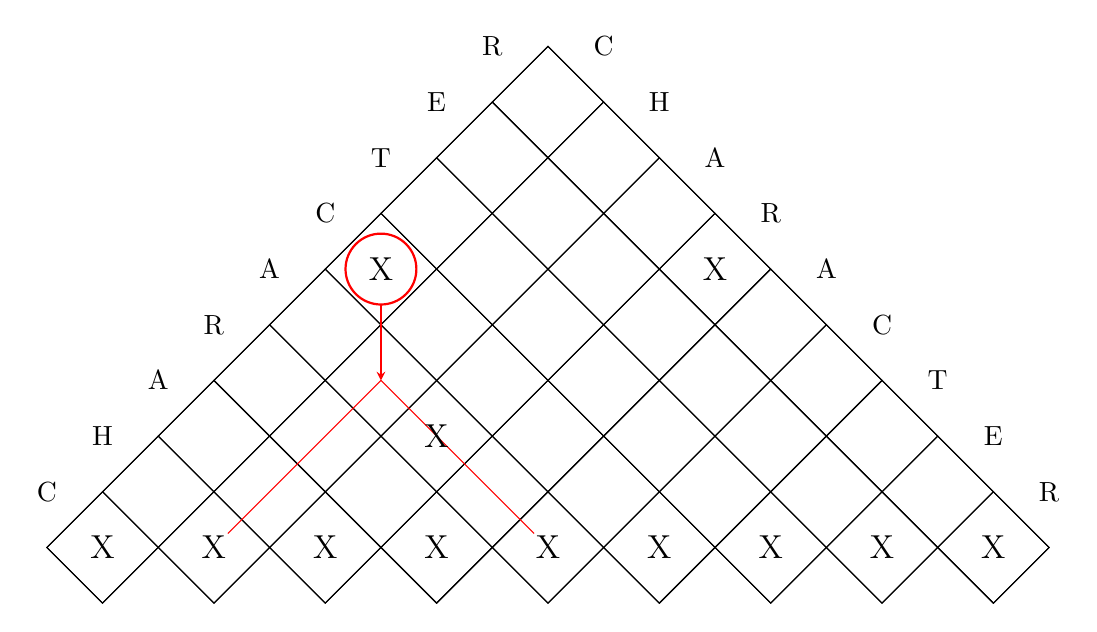
\begin{tikzpicture}[rotate=225]
	\draw (0, 0)  rectangle (1,9);
	\draw (1, 0)  rectangle (2,8);
	\draw (2, 0)  rectangle (3,7);
	\draw (3, 0)  rectangle (4,6);
	\draw (4, 0)  rectangle (5,5);
	\draw (5, 0)  rectangle (6,4);
	\draw (6, 0)  rectangle (7,3);
	\draw (7, 0)  rectangle (8,2);
	\draw (8, 0)  rectangle (9,1);

	\draw (0, 0)  rectangle (9,1);
	\draw (0, 1)  rectangle (8,2);
	\draw (0, 2)  rectangle (7,3);
	\draw (0, 3)  rectangle (6,4);
	\draw (0, 4)  rectangle (5,5);
	\draw (0, 5)  rectangle (4,6);
	\draw (0, 6)  rectangle (3,7);
	\draw (0, 7)  rectangle (2,8);
	\draw (0, 8)  rectangle (1,9);
	\draw [red, thick] (3.5,0.5) circle (0.45cm);
	\draw [->, >=stealth, color=red] (3.81,0.81) -- (4.5,1.5);
	\draw [-, color=red] (4.5,1.5) -- (7.25,1.5);
	\draw [-, color=red] (4.5,1.5) -- (4.5,4.25);

	\node at (-0.5, 0.5) {C};
	\node at (-0.5, 1.5) {H};
	\node at (-0.5, 2.5) {A};
	\node at (-0.5, 3.5) {R};
	\node at (-0.5, 4.5) {A};
	\node at (-0.5, 5.5) {C};
	\node at (-0.5, 6.5) {T};
	\node at (-0.5, 7.5) {E};
	\node at (-0.5, 8.5) {R};

	\node at (0.5, -0.5) {R};
	\node at (1.5, -0.5) {E};
	\node at (2.5, -0.5) {T};
	\node at (3.5, -0.5) {C};
	\node at (4.5, -0.5) {A};
	\node at (5.5, -0.5) {R};
	\node at (6.5, -0.5) {A};
	\node at (7.5, -0.5) {H};
	\node at (8.5, -0.5) {C};

	\node at (0.5, 8.5) {\large X};	
	\node at (0.5, 3.5) {\large X};
	
	\node at (1.5, 7.5) {\large X};
	
	\node at (2.5, 6.5) {\large X};

	\node at (3.5, 5.5) {\large X};
	\node at (3.5, 0.5) {\large X};

	\node at (4.5, 4.5) {\large X};
	\node at (4.5, 2.5) {\large X};

	\node at (5.5, 3.5) {\large X};

	\node at (6.5, 2.5) {\large X};

	\node at (7.5, 1.5) {\large X};

	\node at (8.5, 0.5) {\large X};
\end{tikzpicture}
\end{center}


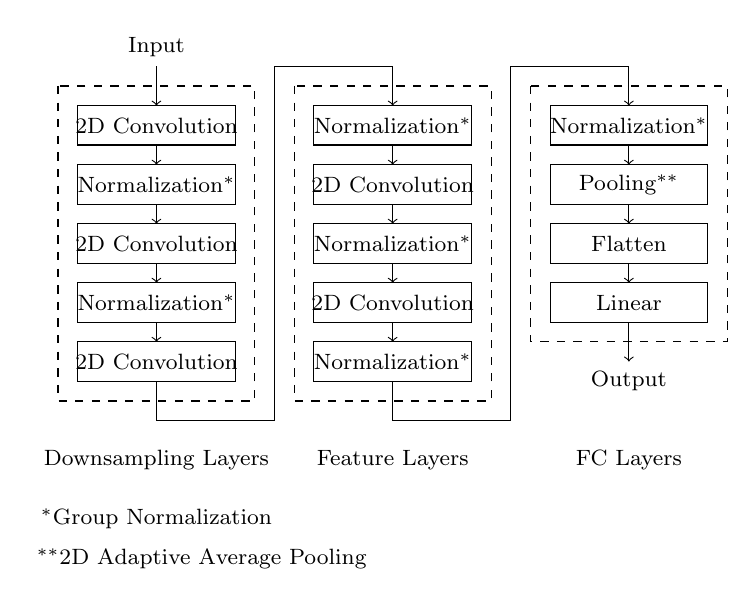
\begin{tikzpicture}
    
%____________________________________________________________________________________________________
    \node[] at (1,-4.5) {\footnotesize{Downsampling Layers}};
    \node[] at (1,0.75) {\footnotesize{Input}};
    \draw[->] (1,0.5) -- (1,0);
    \draw[dashed] (-0.25,0.25) rectangle (2.25,-3.75);
    
    \draw (0,0) rectangle (2,-0.5) node[pos=.5] {\footnotesize{2D Convolution}};
    \draw[->] (1,-0.5) -- (1,-0.75);
    
    \draw (0,-0.75) rectangle (2,-1.25) node[pos=.5] {\footnotesize{Normalization$^{*}$}};
    \draw[->] (1,-1.25) -- (1,-1.5);
    
    \draw (0,-1.5) rectangle (2,-2) node[pos=.5] {\footnotesize{2D Convolution}};
    \draw[->] (1,-2) -- (1,-2.25);
    
    \draw (0,-2.25) rectangle (2,-2.75) node[pos=.5] {\footnotesize{Normalization$^{*}$}};
    \draw[->] (1,-2.75) -- (1,-3);
    
    \draw (0,-3) rectangle (2,-3.5) node[pos=.5] {\footnotesize{2D Convolution}};
    \draw[->] (1,-3.5) -- (1,-4) -- (2.5,-4) -- (2.5,0.5) -- (4,0.5) -- (4,0);
%____________________________________________________________________________________________________
    \node[] at (4,-4.5) {\footnotesize{Feature Layers}};
    \draw[dashed] (2.75,0.25) rectangle (5.25,-3.75);
    
    \draw (3,0) rectangle (5,-0.5) node[pos=.5] {\footnotesize{Normalization$^{*}$}};
    \draw[->] (4,-0.5) -- (4,-0.75);
    
    \draw (3,-0.75) rectangle (5,-1.25) node[pos=.5] {\footnotesize{2D Convolution}};
    \draw[->] (4,-1.25) -- (4,-1.5);
    
    \draw (3,-1.5) rectangle (5,-2) node[pos=.5] {\footnotesize{Normalization$^{*}$}};
    \draw[->] (4,-2) -- (4,-2.25);
    
    \draw (3,-2.25) rectangle (5,-2.75) node[pos=.5] {\footnotesize{2D Convolution}};
    \draw[->] (4,-2.75) -- (4,-3);
    
    \draw (3,-3) rectangle (5,-3.5) node[pos=.5] {\footnotesize{Normalization$^{*}$}};
    \draw[->] (4,-3.5) -- (4,-4) -- (5.5,-4) -- (5.5,0.5) -- (7,0.5) -- (7,0);
%____________________________________________________________________________________________________
    \node[] at (7,-4.5) {\footnotesize{FC Layers}};
    \draw[dashed] (5.75,0.25) rectangle (8.25,-3);
    \draw (6,0) rectangle (8,-0.5) node[pos=.5] {\footnotesize{Normalization$^{*}$}};
    \draw[->] (7,-0.5) -- (7,-0.75);
    
    \draw (6,-0.75) rectangle (8,-1.25) node[pos=.5] {\footnotesize{Pooling$^{**}$}};
    \draw[->] (7,-1.25) -- (7,-1.5);
    
    \draw (6,-1.5) rectangle (8,-2) node[pos=.5] {\footnotesize{Flatten}};
    \draw[->] (7,-2) -- (7,-2.25);
    
    \draw (6,-2.25) rectangle (8,-2.75) node[pos=.5] {\footnotesize{Linear}};
    \draw[->] (7,-2.75) -- (7,-3.25);
    \node[] at (7,-3.5) {\footnotesize{Output}};
    
    \node[] at (1,-5.25) {\footnotesize{$^{*}$Group Normalization}};
    \node[] at (1.575,-5.75) {\footnotesize{$^{**}$2D Adaptive Average Pooling}};
    \end{tikzpicture}

\begin{algorithm}
    \caption{Deep Q-Network with replay buffer}
    \label{fig:pseudo}
    \begin{algorithmic}[1]
        \State Initialize replay memory $\mathcal{D}$ to capacity $N$
        \State Initialize action-value function $Q$ with random weights 
        \For{episode=1,M}
            \State Initialize sequence $s_{1}=\{x_{1}\}$ and preprocessed sequenced $\phi_{1}=\phi(s_{1})$
            \For{t=1,T}
                \State With probability $\epsilon$ select a random action $a_{t}$
                \State otherwise select $a_{t}=\max_{a}Q^{*}(\phi(s_{t}),a;\theta)$
                \State Execute action $a_{t}$ in emulator and observe reward $r_{t}$ and image $x_{t+1}$
                \State Set $s_{t+1}=s_{t},a_{t},x_{t+1}$ and preprocess $\phi_{t+1}=\phi(s_{t+1})$
                \State Store transition $(\phi_{j},a_{j},r_{j},\phi_{j+1})$ in $\mathcal{D}$
                \State Sample random minibatch of transitions $(\phi_{j},a_{j},r_{j},\phi_{j+1})$ from $\mathcal{D}$
                \State Set $y_{j}=
                \begin{cases}
                r_{j} & \text{for terminal }\phi_{j+1}\\
                r_{j}+\gamma\max_{a'}Q(\phi_{j+1},a';\theta) & \text{for non-terminal }\phi_{j+1}
                \end{cases}$
                \State Perform a gradient descent step on $\left(y_{j}-Q(\phi_{j},a_{j};\theta)\right)$ with respect to weights $\theta$
                \State Every $C$ steps reset $\hat{Q}=Q$
            \EndFor
        \EndFor
    \end{algorithmic}
\end{algorithm}

\end{document}






























